\chapter{Revisão Bibliográfica}

O processamento de imagens é uma ferramenta essencial para garantir a confiabilidade do Sistema Elétrico de Potência (SEP), especialmente na detecção e classificação de falhas em equipamentos de linhas de transmissão de energia elétrica. Essa técnica permite identificar problemas em componentes como isoladores, fixadores e suportes, que, se não tratados, podem causar interrupções no fornecimento de energia. O uso de imagens capturadas por drones ou câmeras especiais facilita a inspeção de grandes extensões de linhas de transmissão, reduzindo custos e aumentando a segurança ao evitar a necessidade de intervenções manuais em locais de difícil acesso \cite{eze2022deep}.

Métodos avançados de análise de imagens, como os baseados em aprendizado profundo, ajudam a reconhecer padrões que indicam falhas, mesmo em condições adversas, como baixa visibilidade ou equipamentos desgastados \cite{Altaie2023}. Essas abordagens são particularmente úteis em regiões com infraestrutura antiga, onde a manutenção regular é desafiadora. Além disso, o processamento de imagens possibilita uma resposta rápida a problemas, minimizando o impacto de falhas na rede elétrica e melhorando a continuidade do serviço \cite{kumar2023novel}.

A automação proporcionada pelo processamento de imagens também contribui para a eficiência operacional. Técnicas modernas permitem monitorar equipamentos em tempo real, identificando danos antes que se tornem críticos \cite{eze2022deep}. Isso é crucial para manter a estabilidade do SEP, especialmente em áreas remotas ou com alta demanda energética. Assim, o processamento de imagens não apenas aprimora a manutenção das linhas de transmissão, mas também reforça a segurança e a confiabilidade do fornecimento de energia elétrica.

A seguir, será apresentada uma revisão dos principais conceitos e técnicas de processamento de imagens, que podem ser aplicados na detecção e classificação de falhas em equipamentos de linhas de transmissão de energia elétrica.

\section{Processamento de Imagens}

O processamento de imagens desempenha um papel fundamental no contexto do Sistema Elétrico de Potência (SEP), especialmente em atividades de inspeção, manutenção preditiva e monitoramento de ativos em linhas de transmissão. Com o uso crescente de drones, câmeras térmicas e sensores ópticos, a obtenção de imagens de componentes da rede elétrica tornou-se mais acessível e eficiente. No entanto, a qualidade e a variabilidade dessas imagens exigem técnicas robustas de pré-processamento para garantir resultados precisos em tarefas como a detecção de falhas, corrosões, aquecimentos anômalos e objetos estranhos nas estruturas. Esta seção apresenta os principais métodos de processamento de imagens empregados para preparar dados visuais que serão utilizados em modelos baseados em aprendizado de máquina e redes neurais, contribuindo diretamente para a confiabilidade, segurança e eficiência operacional do SEP.

\subsection{Normalização}
A normalização é uma etapa fundamental no pré-processamento de imagens para redes neurais, pois padroniza os valores dos pixels, facilitando a convergência durante o treinamento e melhorando a generalização do modelo. Um método comum é a normalização de valores de pixels, que escala os valores para intervalos como [0,1] ou [-1,1], frequentemente realizada dividindo os valores originais pelo máximo possível (por exemplo, 255 para imagens de 8 bits) \cite{sharma2024deep}. Outro método é a normalização Z-score, que subtrai a média dos pixels e divide pelo desvio padrão, resultando em dados com média zero e variância unitária \cite{chen2023robustness}. A equalização de histograma também é utilizada para redistribuir as intensidades dos pixels, aumentando o contraste e destacando detalhes em imagens de baixa qualidade \cite{chen2023robustness}. Além disso, a padronização de cores, como subtrair os valores médios dos canais RGB, centraliza os dados em torno de uma distribuição normal, o que é particularmente útil para redes convolucionais \cite{sciencedirect2023normalization}. Técnicas mais avançadas, como a normalização por percentis, utilizam o 5º e o 95º percentis como limites para lidar com valores discrepantes, enquanto a correspondência de histogramas ajusta a distribuição de intensidades com base em pontos de referência \cite{isola2023comparison}. Essas abordagens garantem que as redes neurais processem dados de forma consistente, reduzindo a sensibilidade a variações de iluminação ou escala, especialmente em tarefas de visão computacional \cite{sharma2024deep}.

A Figura \ref{fig:normalizacao} ilustra o processo de normalização de imagens, onde a imagem original é transformada em uma imagem normalizada, facilitando a extração de características relevantes.

\begin{figure}[H]
    \centering
    \caption{\label{fig:normalizacao}Normalização de Imagens}
    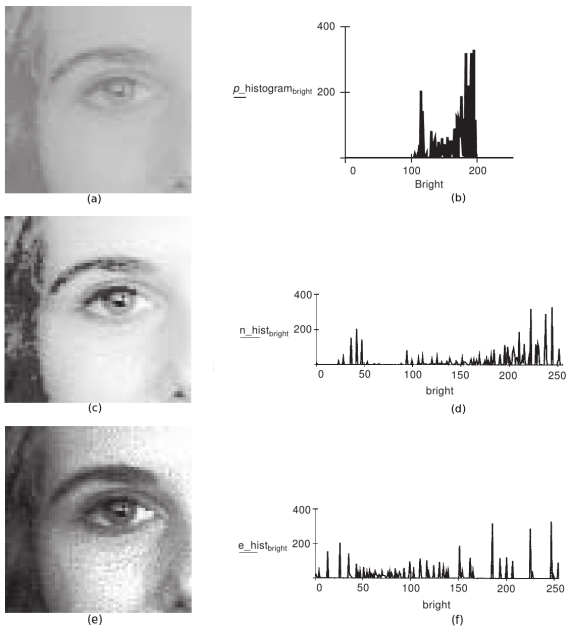
\includegraphics[width=0.8\textwidth]{img/revisao_bibliografica/normalizacao.png}
    \fonte{\citeonline{kuehlkamp2013ferramenta}.}
\end{figure}

\subsection{Redimensionamento e Recorte}
O redimensionamento é essencial para ajustar as imagens ao tamanho de entrada esperado pelas arquiteturas de redes neurais, garantindo compatibilidade e consistência. Um método comum é redimensionar as imagens para um tamanho fixo, como 224x224 pixels, amplamente utilizado em modelos como ResNet e VGG \cite{chen2023robustness}. Isso pode ser feito por meio de interpolação bilinear ou bicúbica, que suaviza as transições entre pixels, embora métodos mais avançados, como interpolação baseada em Fourier, também sejam explorados \cite{dennanni2019resizing}. O recorte, por outro lado, extrai uma região de interesse da imagem, frequentemente centrada, para preservar áreas relevantes, especialmente quando as dimensões originais variam significativamente \cite{sciencedirect2023normalization}. Estudos indicam que o redimensionamento para tamanhos menores pode acelerar o treinamento, mas tamanhos muito reduzidos podem comprometer a qualidade das características extraídas \cite{sabottke2020effect}. Além disso, o recorte aleatório é usado em conjunto com aumento de dados para introduzir variabilidade durante o treinamento \cite{nalepa2022data}. Essas técnicas são cruciais para lidar com conjuntos de dados heterogêneos, garantindo que as entradas sejam uniformes sem perda significativa de informação \cite{chen2023robustness}.

A Figura \ref{fig:redimensionamento_e_recorte} ilustra o processo de redimensionamento e recorte de imagens, na qual a imagem da esquerda (original) é utilizada para extrair uma região de interesse (recorte) e em seguida redimensionada para um tamanho fixo (imagem da direita).

\begin{figure}[H]
    \centering
    \caption{\label{fig:redimensionamento_e_recorte}Redimensionamento e recorte}
    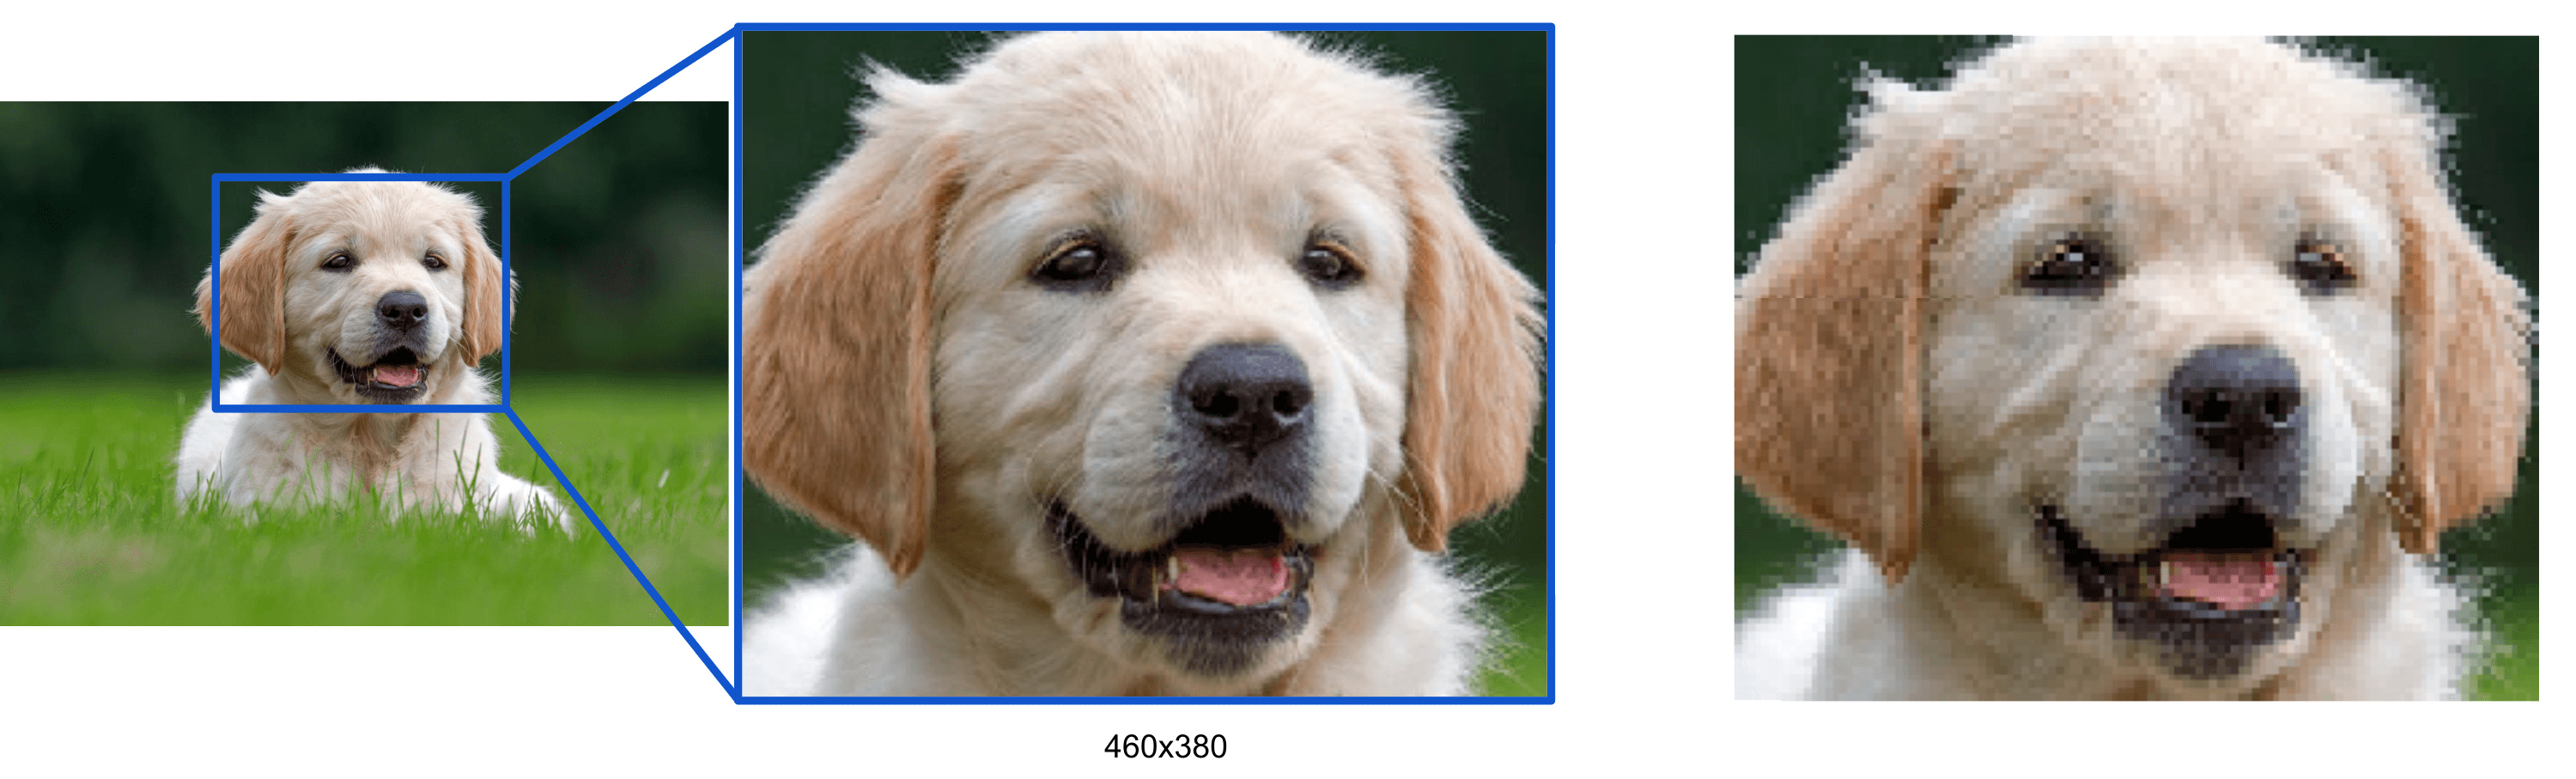
\includegraphics[width=1\textwidth]{img/revisao_bibliografica/redimensionamento_e_recorte.png}
    \fonte{Adaptado de \citeonline{venturelli2021}.}
\end{figure}

\subsection{Aumento de Dados}
O aumento de dados é uma estratégia poderosa para ampliar a diversidade do conjunto de treinamento, reduzindo o risco de sobreajuste e melhorando a robustez do modelo. Técnicas geométricas incluem espelhamento horizontal ou vertical, rotações em ângulos variados (de 1° a 359°), translações, cortes aleatórios e ajustes de escala, que simulam diferentes perspectivas e tamanhos \cite{shorten2019survey}. Transformações no espaço de cores, como ajustes de brilho, contraste, saturação e matiz, ajudam a lidar com variações de iluminação \cite{shorten2019survey}. Métodos mais avançados, como apagamento aleatório, mascaram partes da imagem para simular oclusões, enquanto a mistura de imagens combina pixels de diferentes amostras para criar novas instâncias \cite{shorten2019survey}. Por exemplo, o método SamplePairing reduziu o erro no conjunto CIFAR-10 de 8,22\% para 6,93\% \cite{shorten2019survey}. Além disso, redes adversárias generativas (GANs) são usadas para gerar imagens sintéticas, especialmente em domínios com dados limitados, como imagens médicas, alcançando melhorias de até 10\% em precisão \cite{shorten2019survey}. Essas técnicas são particularmente valiosas em cenários com poucos dados, permitindo que as redes neurais generalizem melhor para condições não vistas \cite{nalepa2022data}.

\subsection{Redução de Ruído}
A redução de ruído remove interferências que podem comprometer o desempenho das redes neurais, sendo especialmente crítica em aplicações como imagens médicas e vigilância. Métodos tradicionais, como filtros de média ou mediana, são complementados por abordagens baseadas em aprendizado profundo, como redes neurais convolucionais (CNNs) especializadas, como DnCNNs, que aprendem a mapear imagens ruidosas para versões limpas \cite{sharma2024deep}. Autoencoders também são empregados para reconstruir imagens a partir de representações latentes, eliminando ruídos como Gaussianos ou de sal e pimenta \cite{sharma2024deep}. Técnicas como Total Variation Denoising (TVD) e Non-Local Means (NLM) exploram regularizações e similaridades entre pixels para preservar detalhes \cite{sharma2024deep}. Um estudo demonstrou que a aplicação de DnCNNs em imagens de tomografia computadorizada resultou em uma precisão de detecção de câncer de pulmão variando de 86,17\% a 99,67\% \cite{sharma2024deep}. Além disso, métodos baseados em redes neurais profundas, como o Deep Neural Filter (DNF), alcançaram melhorias de até 10 dB na relação sinal-ruído em sinais de EEG \cite{peer2022real}. Essas abordagens são essenciais para garantir que as redes neurais processem imagens de alta qualidade, minimizando artefatos que poderiam obscurecer características críticas \cite{sharma2024deep}.

A Figura \ref{fig:reducao_de_ruido} ilustra o processo de redução de ruído, onde a imagem original (à esquerda) é processada para remover o ruído, resultando em uma imagem mais limpa (à direita).

\begin{figure}[H]
    \centering
    \caption{\label{fig:reducao_de_ruido}Redução de Ruído}
    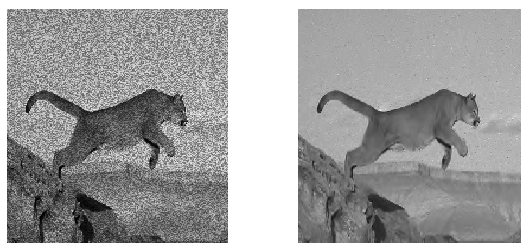
\includegraphics[width=1\textwidth]{img/revisao_bibliografica/reducao_de_ruido.png}
    \fonte{Adaptado de \citeonline{wavelet_denoising}.}
\end{figure}

\subsection{Ajuste de Contraste e Brilho}
O ajuste de contraste e brilho melhora a visibilidade das características das imagens, sendo crucial para tarefas que dependem de detalhes finos. A equalização de histograma redistribui as intensidades dos pixels para maximizar o contraste, enquanto a equalização adaptativa limitada por contraste (CLAHE) evita a amplificação excessiva de ruído em regiões homogêneas \cite{sciencedirect2023normalization}. A correção gama ajusta a curva de intensidade para realçar detalhes em áreas escuras ou claras, sendo amplamente usada em imagens de baixa qualidade \cite{sciencedirect2023normalization}. Métodos baseados em aprendizado profundo, como redes convolucionais fuzzy, integraram filtros Gaussianos e triangulares para melhorar imagens de íris, alcançando até 97\% de precisão em tarefas de reconhecimento \cite{sharma2024deep}. Além disso, técnicas como RetinexDIP foram propostas para melhorar a resolução e reduzir o consumo de memória em comparação com métodos tradicionais \cite{sharma2024deep}. Essas abordagens são fundamentais para preparar imagens para redes neurais, garantindo que as características relevantes sejam destacadas \cite{sciencedirect2023normalization}.

% imagem de exemplo do CLAHE. cite isso no texto abaixo
A Figura \ref{fig:clahe} ilustra o efeito do CLAHE em uma imagem, destacando detalhes que antes estavam obscurecidos.

\begin{figure}[H]
    \centering
    \caption{\label{fig:clahe}Ajuste de Contraste e Brilho com CLAHE}
    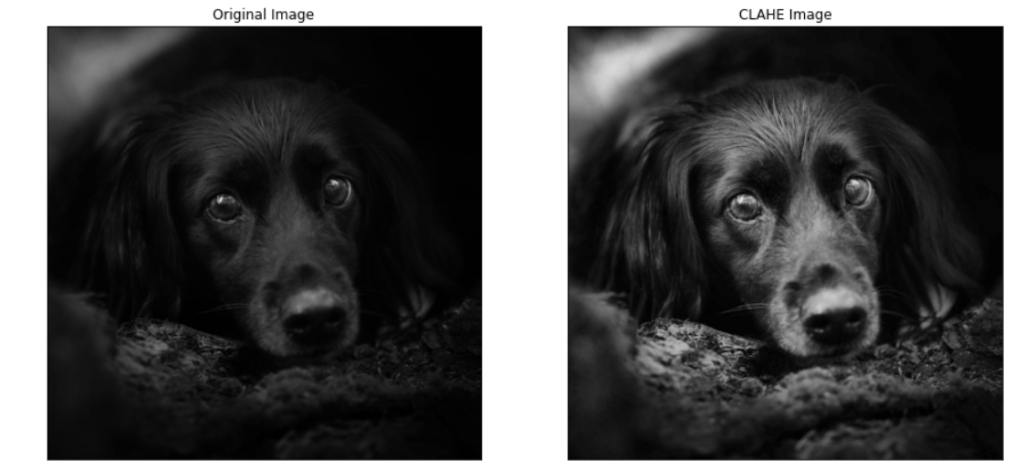
\includegraphics[width=1\textwidth]{img/revisao_bibliografica/clahe.png}
    \fonte{\citeonline{pandey2023image}.}
\end{figure}

\subsection{Aumento de Nitidez}
O aumento de nitidez realça bordas e detalhes finos, facilitando tarefas como detecção de objetos e segmentação. Técnicas tradicionais, como a máscara de desfoque, aplicam filtros de alta passagem para enfatizar transições de intensidade \cite{sciencedirect2023normalization}. Métodos baseados em redes neurais, como CNNs, foram desenvolvidos para detectar e corrigir nitidez, como no caso da detecção de máscaras de desfoque (USM), superando métodos baseados em codificação ternária perpendicular a bordas \cite{ding2018detecting}. Em aplicações específicas, como imagens de documentos, redes convolucionais combinadas com filtros de Gabor e desfoque melhoraram a legibilidade, reduzindo distorções como sombras e ruídos \cite{ben2022deep}. Essas técnicas são particularmente úteis em cenários onde a clareza das bordas é essencial para o desempenho do modelo \cite{sharma2024deep}.

A Figura \ref{fig:aumento_de_nitidez} ilustra o efeito do aumento de nitidez em uma imagem, onde os detalhes são mais evidentes após o processamento.

\begin{figure}[H]
    \centering
    \caption{\label{fig:aumento_de_nitidez}Aumento de Nitidez}
    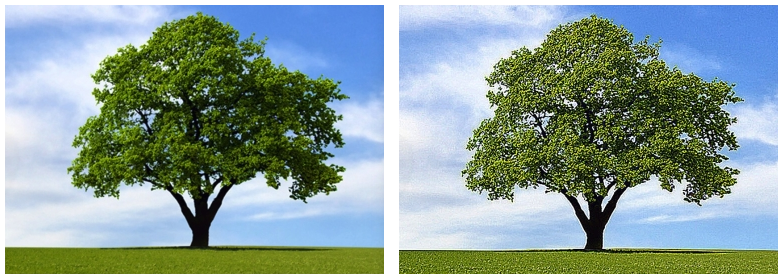
\includegraphics[width=1\textwidth]{img/revisao_bibliografica/aumento_de_nitidez.png}
    \fonte{Adaptado de \citeonline{joshi2025}.}
\end{figure}

\subsection{Conversão de Espaço de Cores}
A conversão de espaço de cores adapta as imagens às necessidades específicas da tarefa, simplificando o processamento ou destacando características relevantes. A conversão de RGB para escala de cinza reduz a dimensionalidade, sendo útil em tarefas onde a cor não é essencial \cite{sharma2024deep}. Espaços como HSV e LAB são preferidos em aplicações que requerem separação de matiz, saturação ou luminância, como segmentação de objetos \cite{sharma2024deep}. Redes neurais também foram usadas para realizar conversões de espaço de cores, como de RGB para XYZ, alcançando erros de cor inferiores a 1,0 unidade ΔE 2000 em mais de 85\% dos casos testados \cite{macdonald2019color}. Essas conversões são valiosas para otimizar a extração de características e reduzir a complexidade computacional em tarefas de visão computacional \cite{sharma2024deep}.

\subsection{Restauração e Desembaçamento de Imagens}
A restauração de imagens visa recuperar a imagem original a partir de versões degradadas por desfoque, ruído ou outras distorções. O desembaçamento, um subcampo da restauração, utiliza redes neurais como U-Net para corrigir desfoques dinâmicos, alcançando PSNR de 31,53 no conjunto GoPro e 31,32 no Real Blur \cite{Lian2023Deblurring}. Métodos baseados em autoencoders convolucionais foram propostos para restaurar imagens em aplicações de fotografia computacional e sensoriamento remoto \cite{barreto2020cnn}. Além disso, redes neurais como DnCNNs foram aplicadas para remover ruídos específicos, como speckle em imagens holográficas \cite{sharma2024deep}. Essas técnicas são cruciais para preparar imagens de alta qualidade para redes neurais, especialmente em domínios onde a clareza é essencial \cite{sumida2019deep}.

A Figura \ref{fig:desembacamento} ilustra o processo de desembaçamento, onde a imagem original (à esquerda) é processada para remover o desfoque, resultando em uma imagem mais nítida (à direita).

\begin{figure}[H]
    \centering
    \caption{\label{fig:desembacamento}Restauração e Desembaçamento de Imagens}
    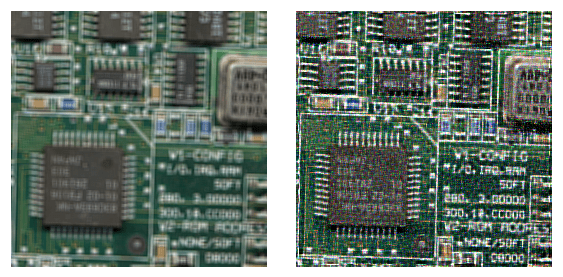
\includegraphics[width=1\textwidth]{img/revisao_bibliografica/desembacamento.png}
    \fonte{Adaptado de \citeonline{mathworks2025lucyrichardson}.}
\end{figure}

\subsection{Detecção de Bordas}
A detecção de bordas identifica limites e formas nas imagens, sendo uma etapa fundamental em muitas tarefas de visão computacional. Redes neurais, como redes de codificação-decodificação, foram desenvolvidas para detectar bordas com alta precisão, superando detectores tradicionais como Canny em imagens ruidosas \cite{yu1994edge}. Métodos inspirados em mecanismos biológicos, como redes com atenção seletiva, melhoraram a extração de características globais, resultando em mapas de bordas mais robustos \cite{chen2022edge}. Essas abordagens são essenciais para pré-processar imagens, fornecendo informações estruturais que facilitam a segmentação e o reconhecimento de objetos \cite{yu1994edge}.

A Figura \ref{fig:deteccao_de_bordas} ilustra o processo de detecção de bordas, onde as bordas da imagem original (à esquerda) são destacadas na imagem processada (à direita).

\begin{figure}[H]
    \centering
    \caption{\label{fig:deteccao_de_bordas}Detecção de Bordas}
    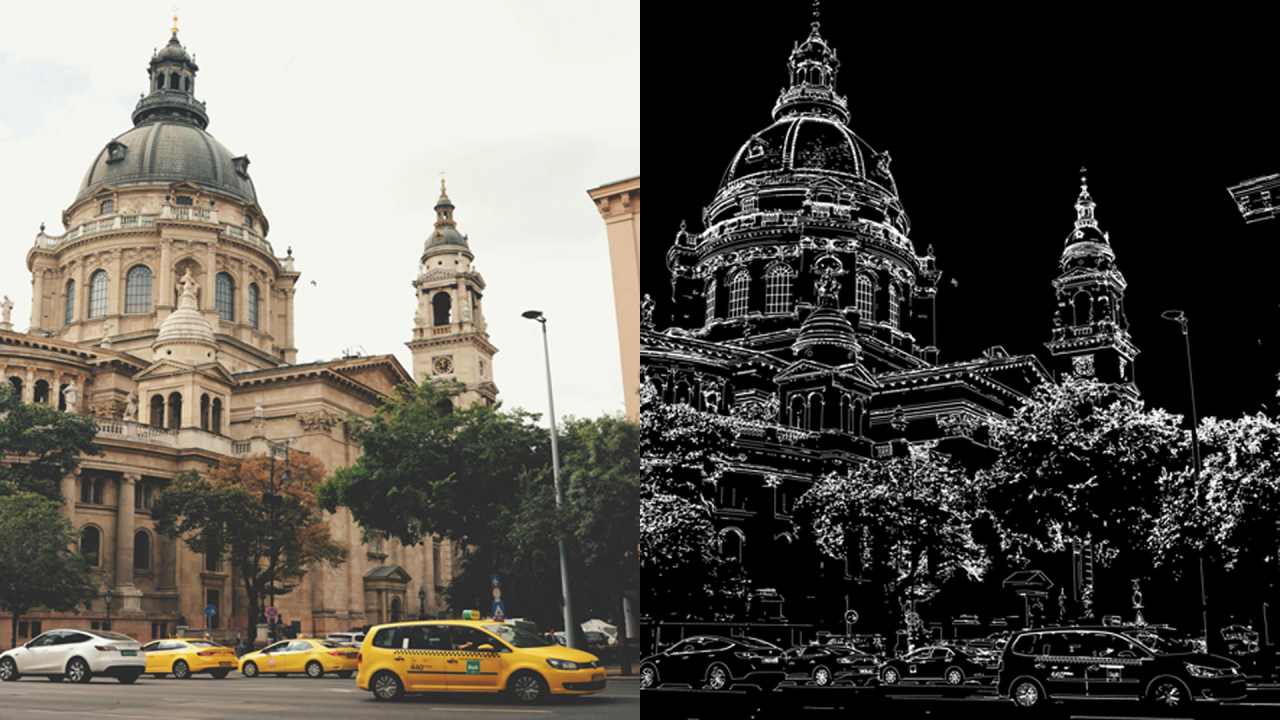
\includegraphics[width=1\textwidth]{img/revisao_bibliografica/deteccao_de_bordas.png}
    \fonte{\citeonline{couto2024regions}.}
\end{figure}

\subsection{Correção de Iluminação}
A correção de iluminação normaliza as condições de luz nas imagens, garantindo consistência na extração de características. Métodos baseados em aprendizado profundo, como redes convolucionais, foram propostos para corrigir imagens com iluminação desigual, como pinturas, alcançando resultados superiores em métricas como NIQE e LOE \cite{li2020simple}. Técnicas híbridas que combinam modelos baseados em aprendizado e físicos foram aplicadas para melhorar a detecção de objetos em condições de luz variada, como em imagens de plantações \cite{yang2022using}. Essas abordagens são particularmente úteis em cenários onde a iluminação não uniforme pode comprometer o desempenho do modelo \cite{li2020simple}.

A Figura \ref{fig:correcao_de_iluminacao} ilustra o processo de correção de iluminação, onde a imagem original (à esquerda) é processada para uniformizar a iluminação, resultando em uma imagem mais equilibrada (à direita).

\begin{figure}[H]
    \centering
    \caption{\label{fig:correcao_de_iluminacao}Correção de Iluminação}
    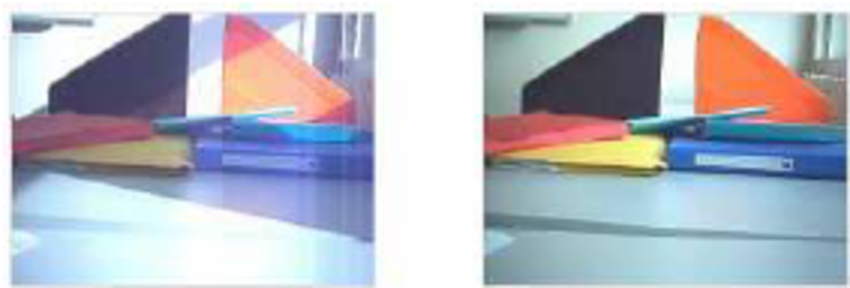
\includegraphics[width=1\textwidth]{img/revisao_bibliografica/correcao_de_iluminacao.png}
    \fonte{\citeonline{Bascle2006IlluminationCorrection}.}
\end{figure}

\subsection{Super-Resolução}
A super-resolução aumenta a resolução de imagens, gerando versões de alta qualidade a partir de entradas de baixa resolução. Redes neurais, como redes convolucionais profundas e redes adversárias generativas (GANs), alcançaram resultados impressionantes, com modelos como SRGAN produzindo imagens fotorrealistas \cite{ledig2017photo}. Em aplicações biológicas, redes como DPA-TISR foram desenvolvidas para imagens de células vivas, alcançando fidelidade temporal e consistência em mais de 10.000 pontos temporais \cite{liu2025neural}. Essas técnicas são valiosas para tarefas que requerem detalhes finos, como análise médica e vigilância, permitindo que redes neurais processem imagens com maior clareza \cite{ledig2017photo}.

\subsection{Conclusão parcial da seção}

O processamento de imagens é uma etapa crucial para garantir a eficácia dos modelos de aprendizado profundo aplicados ao Sistema Elétrico de Potência (SEP). As técnicas discutidas, como normalização, redimensionamento, aumento de dados e redução de ruído, podem ser fundamentais para preparar as imagens antes de serem alimentadas em redes neurais. Essas abordagens não apenas melhoram a qualidade das imagens, mas também garantem que os modelos sejam mais robustos e capazes de generalizar em diferentes condições. A escolha adequada dessas técnicas pode impactar significativamente o desempenho dos modelos na detecção e classificação de falhas em equipamentos de linhas de transmissão.

\section{Redes Neurais}
Aqui, serão discutidos os diferentes tipos de redes neurais aplicáveis ao processamento de imagens, com foco em suas arquiteturas e aplicações específicas para avaliação de desempenho.

\subsection{Métricas}
Serão apresentadas as principais métricas utilizadas para avaliar a eficácia dos processamentos de imagem, como acurácia, tempo de processamento, precisão, recall, entre outras.

\section{Métodos de Ajuste de Parâmetros e Combinação de Processamentos}
Serão explorados os métodos para ajuste automático de parâmetros e a combinação de diferentes técnicas de processamento de imagem para otimização dos resultados.
